\makeatletter\let\ifGm@compatii\relax\makeatother
\documentclass[final, %
	% 10pt, % slightly smaller
	%11pt, % standard font size
	% 12pt, % slightly bigger
	% handout, % for producing handouts
	t, % Place text of slides at the (vertical) top of the slides
	% c, % Place text of slides at the (vertical) center of the slides
	xcolor={table,dvipsnames}, % options for xcolor
]{beamer}


%%%%%%%%%%%%%%%%%%%%%%%%%%%%%%
% my theme design is in style.sty file. Go there and see my comments
\usepackage{style}


%%%%%%%%%%%%%%%%%%%%%%%%%%%%%%

\usepackage{etex}
\usepackage[utf8]{inputenc}
\usepackage{graphicx}
\usepackage[T1]{fontenc} % for correct hyphenation of words with accented letters in European languages 
\usepackage{textcomp}	 % additional symbols (Text Companion font extension)

% \usepackage{lmodern}               %% --- Latin Modern
\usepackage{mathptmx}              %% --- Times mit Matheschriften
\usepackage{multirow}
% \usepackage{mathpazo}              %% --- Palatino

\usepackage[scaled=.90]{helvet}    %% --- Helvetica (Arial)
\usepackage{rotating}


\usepackage{courier}               %% --- Courier
\usepackage{amsmath}
% preamble/Beamer-LaTeX-Settings.tex
% pictures
\usepackage[%
  %final,
   %draft % do not include images (faster)
]{graphicx}
		


\usepackage{tabularx}   % enables more options for tables
\usepackage{booktabs}
\usepackage{multicol}

% 
\usepackage[absolute,overlay]{textpos}


%%package for braces\usetikzlibrary{decorations.pathreplacing}

%%package for bar charts
\usepackage{pgfplots}

%% use ellipse as node
\usetikzlibrary{arrows}
\usetikzlibrary{shapes}

\usepackage{amsmath}
% for adding python source code to latex
\usepackage{listings}


%%%%%%%%%%%%%%%%%%%%%%%%%%%%%
\title{Deep Learning for NLP \\
Lecture 4: Text Representations I 
}

\author{\LARGE{Dr. Mohsen Mesgar} \\
\vspace{0.5cm}
\normalsize{Ubiquitous Knowledge Processing Lab (UKP Lab)}}
\date{}
%%%%%%%%%%%%%%%%%%%%%%%%%%%%%
\begin{document}
\begin{frame}
\titlepage
\end{frame}

\begin{frame}{This lecture}
\vspace*{1cm}

\begin{itemize}
        \item common features used for converting textual data into numerical vectors
        \item basics of word embeddings
            \begin{itemize}
                \item how to get them? 
                \item where to use them?
                \item how to use them?
            \end{itemize}
        \item limitations
\end{itemize}
\end{frame}
%%%%%%%%%%%%%%%%%%%%%%%%%%%%%%%%
\begin{frame}{Recall}
    \begin{itemize}
        \item<1-> the input to a supervised learning algorithm is a training set ($x_{1:n}, y_{1:n}$), where
        \begin{itemize}
            \item<2-> $x_{1:n} = x_1,x_2,..., x_n$ shows input examples
            \item<3->  $y_{a:n}= y_1, y_2, ..., y_n$ shows corresponding labels
        \end{itemize}
        \item<4-> the goal of a learning algorithm is to return a function $f()$ that accurately maps input examples to their desired labels
        \uncover<5->{
        \begin{figure}
\centering
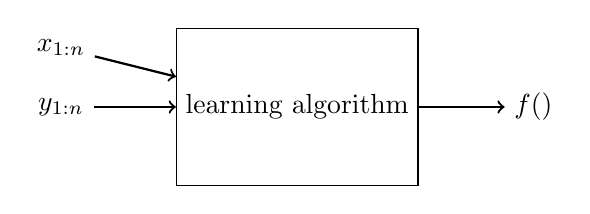
\begin{tikzpicture}

\node(x) at (0, 0) [] {$x_{1:n}$};
\node(y) at (0, -0.75) [] {$y_{1:n}$};


\node(lr) at (3,-0.75) [draw, minimum width=2cm, minimum height=2cm]{learning algorithm};

\draw[->,thick] (x) to (lr);
\draw[->,thick] (y) to (lr);

\node(f) at (6.0, -0.75) [] {$f()$};
\draw[->,thick] (lr) to (f);

\end{tikzpicture}
\end{figure}
        }
        \item<7-> the input to neural models $f()$ should be a numerical vector but NLP tasks are defined on texts
        \item<8-> how can we represent texts via numerical vectors? 
    \end{itemize}
\end{frame}
\begin{frame}{Text Representation \\ (a.k.a., Feature Extraction)}
    \begin{itemize}
        \item<1->  vector representation of a text should ideally reflect various linguistic properties of the text
        \item<2-> 
        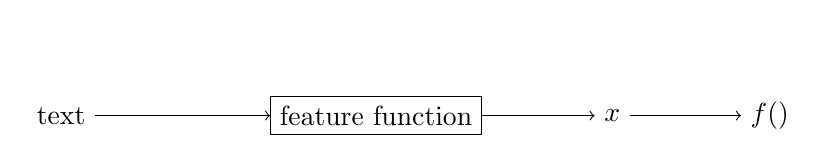
\begin{tikzpicture}
        \node[] () at (0,1) {};
        \node[] (text) at (0,0) {text};
        \node[draw] (feat_ext) at (4,0) {feature function};
        \node[] (x) at (7,0) {$x$};
        \node[] (f) at (9,0) {$f()$};
        
        
        \draw[->] (text) -- (feat_ext);
        \draw[->] (feat_ext) -- (x);
        \draw[->] (x) -- (f);
        \end{tikzpicture}  
        \item<3-> in this lecture we focus on  feature functions rather than learning algorithms
    \end{itemize}
\end{frame}

\begin{frame}{Some Terminologies}
    \begin{itemize}
        \item<1-> letters: smallest units in a language $\rightarrow$ a,b,c,...
        \item<2-> tokens and words: tokens are outputs of a tokenizer and words are meaning-bearing units
        \begin{itemize}
            \item note: in this course we use the terms ``word" and ``token" interchangeably 
        \end{itemize}
        \item<3-> lemma: the dictionary entry of the word $\rightarrow$ ``book" is the lemma of ``booking", ``booked", and ``books"
            \begin{itemize}
                \item how to obtain lemmas? use morphological analyzers 
                \item are available for many languages
                \item lemmatization may not work for any sequence of letters e.g., for mis-spelling
            \end{itemize}
            
        \item<4-> stems: a shorter venison of a word defined based on some language-specific heuristic $\rightarrow$ ``pictur'' is the stem of ``pictures'', ``pictured'', and ``picture''
        \begin{itemize}
            \item the output of a stemmer need not be a valid word
        \end{itemize}
    \end{itemize}
\end{frame}
\begin{frame}{Some Terminologies}
    \begin{itemize}
        \item lexical resources: provide some information about words and their relations
        \begin{itemize}
            \item<1-> dictionaries
            \item<2-> WordNet for English
                \begin{itemize}
                    \item<3-> capture semantic knowledge about words
                    \item<4-> each word is associated with one or several synsets
                    \item<5-> synsets are linked to each other according to semantic relations  between their words
                    \item<6-> semantic relations are: hypernym (more specific),  hyponym (less specific), antonyms, holonyms (part-whole), and meronyms (whole-part) 
                    \item<7-> contains information about nouns, verbs, adjectives, and adverbs
                    \item<8-> manually created
                \end{itemize}
            \item<9-> FrameNet and VerbNet for English
            \begin{itemize}
                \item<10-> focus around verbs
                \item<11-> manually created
            \end{itemize}
            \item<12-> Paraphrase Database (PPDB) 
            \begin{itemize}
                \item<13-> contains paraphrases 
                \item<14-> automatically created
            \end{itemize}
        \end{itemize}
    \end{itemize}
\end{frame}
\begin{frame}{Common Features for Textual Data}
    what information can  we extract directly from  a word 
    \begin{itemize}
        \item<1-> letters comprising a word and their order
        \item<2-> length of word
        \item<3-> is the first letter capitalized?
        \item<4-> does word include hyphen? 

    \end{itemize}
    
\end{frame}
\begin{frame}{Common Features for Textual Data}
    \begin{itemize}
        \item<1-> Bag-of-Words (BoW): the count of each word in a text is taken as a feature
            \begin{figure}
                \centering
                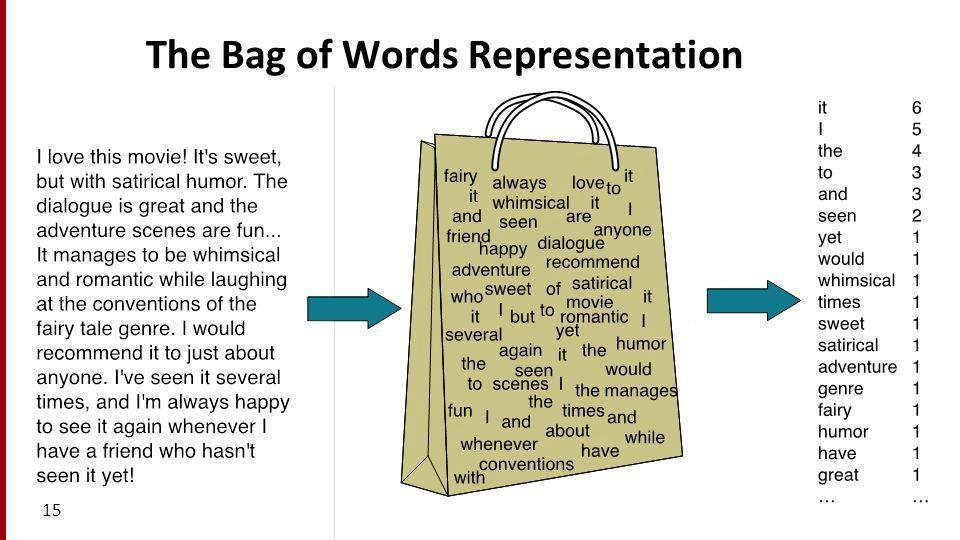
\includegraphics[scale=0.25]{./figure/bow.jpg}
            \end{figure}
    \item<2-> BOW does not care about the order of words
    \end{itemize}
    
    
    \vspace*{\fill}
     \textit{\tiny{(Taken from:\url{https://www.programmersought.com/article/4304366575/)}}}
\end{frame}
\begin{frame}{Common Features for Textual Data}
    \begin{itemize}
        \item<1-> TF-IDF: Term Frequency - Inverse Document Frequency
        \item<2-> let $d$ be a document from a given corpus $D$
        \item<3-> we map word $w$ of $d$ to a number as follows:
        
        \begin{equation*}
            \frac{\#(w,d)}{\sum_{w^\prime}  \#(w^\prime, d)} \times \text{log}\frac{|D|}{|\{ d\in D: w \in d\}|}
        \end{equation*}
        \item<4-> N-grams: instead of using the frequency of a word, we use the frequency of N sequence of words 
        \item<5-> N=2 $\rightarrow$ bi-gram 
        \item<6-> N=3 $\rightarrow$ tri-gram
    \end{itemize}
\end{frame}
\begin{frame}{Common Features for Textual Data}
\begin{itemize}
\item<1-> context: each piece of a text occurs within a larger text which is known as context
\item<2-> how to encode contextual information?
    \item<3-> using position of a word within a sentence or a document
    \item<4-> using the words that appear in an immediate context of a word
    \begin{itemize}
        \item<5-> immediate context: a window of $k$ words surrounding the target word
        \item<6-> ``the cat \underline{sat} on the mat'' , $k$=2 $\rightarrow$ $\{$ word-minus-2=the, word-minus-1=cat, word-plus-1=on, word-plus-2=the $\}$
    \end{itemize}
\end{itemize}
\end{frame}
\begin{frame}{Common Features for Textual Data}
    what information can we extract from the relation of text with external source of information?
    \begin{itemize}
        \item<1-> is a word in a list of common person names in Germany? 
        \item<2-> is a word a female or male person name?
        \item<3-> what is the lemma of the word?
        \item<4-> what is the stem of the word?
        \item<5-> what information do lexical resources give us about the word?
    \end{itemize}
\end{frame}
\begin{frame}{Feature Vectors}
    \begin{itemize}
        \item<1-> the output of a learning algorithm is a $f()$
        \item<2-> $f$ takes as input a vector $x$ with dimension $d_{in}$
        \item<3-> $f$ returns as output a vector $\hat{y}$ with dimension $d_{out}$
        \item<4-> how can we map textual features to a vector?
    \end{itemize}
\end{frame}
\begin{frame}{Different Types of Features}
    \begin{itemize}
        \item<1-> numerical features 
        \begin{itemize}
            \item<1-> the value of a feature is a number 
            \item<2-> e.g., the frequency of a word in a text
        \end{itemize}
        \item<3-> categorical features
        \begin{itemize}
            \item<3-> the value of a feature is from a set of values
            \item<4-> what is the POS of a word? 
        \end{itemize}
        
        \item<5-> how to encode categorical features?
        \begin{itemize}
            \item<6-> one-hot encodings
            \item<7-> dense embeddings
        \end{itemize}
        
    \end{itemize}
\end{frame}
\begin{frame}{One-hot Encodings}  
    \begin{itemize}
        \item<1-> let's assume that values of a feature is in categories $\{ v_0, v_1, v_2 \}$
        \item<2-> we encode the space of feature values via vectors in which 
            \begin{itemize}
                \item<3-> each entry is either $0$ or $1$
                \item<4-> each entry is associated with one of the categories
                \item<5-> only one item in a vector can be $1$, the rest should be $0$
            \end{itemize}
        \item<6-> for example:
        \begin{itemize}
            \item<6-> $v_0 = [1, 0, 0]$
            \item<6-> $v_1 = [0, 1, 0]$
            \item<6-> $v_2 = [0, 0, 1]$
        \end{itemize}
    \end{itemize}
\end{frame}
\begin{frame}{Example: Categorical Labels}
    \begin{itemize}
        \item<1-> let $f()$ take a vector $x$ which encodes a text and also return a vector $\hat{y}$ representing the topic of the text which can be from $\{$news, sport, science, politic$\}$
        \item<2-> how can we represent topic labels using one-hot encoding? 
        \begin{itemize}
            \item<3-> news = $[1,0,0,0]$
            \item<4-> sport = $[0,1,0,0]$
            \item<5-> science = $[0,0,1,0]$
            \item<6-> politic = $[0,0,0,1]$
        \end{itemize}
        \item<7-> what is the length of one-hot vectors for a feature with $k$ categories?  
        
    \end{itemize}
\end{frame}
\begin{frame}{Example: Word Encodings}
    \begin{itemize}
        \item<1-> let $V$ be vocabulary of a language 
        \item<2-> we take $V$ as categories a word can take in a text
        \item<3-> so words can be encoded by one-hot vectors
        \item<4-> let $V= \{v_0, v_1, v_2,...,v_{|V|-1} \}$
        \begin{itemize}
            \item<5-> $v_0 = [1,0,0,..., 0]$
            \item<6-> $v_1 = [0,1,0,..., 0]$
            \item<7-> $v_2 = [0,0,1,..., 0]$
            \item<7-> $...$
            \item<7-> $v_{|V|-1} = [0,0,0,..., 1]$
        \end{itemize}
        \item<8-> we can easily represent a text via BOW and then represent each word in BOW with its one-hot vector
        \item<9-> how can we define vocabulary $V$ given a corpus $D$?
    \end{itemize}
\end{frame}

\begin{frame}{Comment}
    \centering
    \textcolor{myblue}{\Large{\textbf{pause}}}
\end{frame}


\begin{frame}{One-hot Encodings}
\begin{itemize}
    \item<1-> word vectors are very sparse 
    \item<2-> semantic relations between words are not encoded in word vectors
    \item<3-> it's better to use one-hot representations for a few distinct features where we expect no correlation between features
\end{itemize}\end{frame}

\begin{frame}{Dense Encodings}
    \begin{itemize}
        \item<1-> a categorical feature is embedded as a vector in a $d$ dimensional space
        \item<2-> assuming categories $C = \{ c_0,c_1,..., c_{|C|-1} \}$, $d=4$
        \begin{itemize}
            \item<3-> $c_0 = [+0.1,-0.2,+0.3,+0.5]$
            \item<4-> $c_1 = [-0.2-0.1,+0.1,+0.2]$
            \item<4-> ...
            \item<4-> $c_{|C|-1} = [+0.2,-0.2,-0.1,+0.3]$
        \end{itemize}
    \end{itemize}
\end{frame}
\begin{frame}{Example: Word Encodings}
    \begin{itemize}
        \item<1-> assuming vocabulary $V = \{ v_0,v_1,..., v_{|V|-1} \}$, $d=4$
        \begin{itemize}
            \item<2-> $v_0 = [+0.1,-0.2,+0.3,+0.5]$
            \item<2-> $v_1 = [-0.2-0.1,+0.1,+0.2]$
            \item<2-> ...
            \item<2-> $v_{|V|-1} = [+0.2,-0.2,-0.1,+0.3]$
        \end{itemize}
        \item<3-> in the one-hot method we represent each word with a sparse vector of size $|V|$
        \item<4-> in dense encoding method we represent each word with a dense vector with a small size $d$
    \end{itemize}
\end{frame}
\begin{frame}{Dense Encodings}
    \begin{itemize}
        \item<1-> dimensionality of vectors is $d$
        \item<2-> model training will cause similar features to have similar vectors
        \item<3-> it's mainly useful when we expect some correlations between features $\rightarrow$ ``cat'' and ``dog'' are semantically related
        \item<4-> is also useful when we have a large number of features $\rightarrow$ for example vocabulary
    \end{itemize}
\end{frame}
\begin{frame}{Embeddings}
    \begin{itemize}
        \item<1-> by embeddings we mean representing each textual feature as a dense vector in a low dimensional space
        \item<2-> how should we define these dense vectors or embeddings?
    \end{itemize}
\end{frame}
\begin{frame}{Word Embeddings}
    \begin{itemize}
        \item dense representations of words in an embedding space is known as word embeddings
        \item how to obtain word embeddings?  
    \end{itemize}
\end{frame}
\begin{frame}{Random Initizalization}
    \begin{itemize}
        \item<1-> we initialize the embedding vectors to random values
        \item<2-> values are uniformly sampled from numbers in the range
        \begin{itemize}
            \item<3->  $[-\frac{1}{2d}, +\frac{1}{2d} ] $ where $d$ is the number of dimensions (Mikolov et al., 2013)
            \item<4->  $[-\frac{\sqrt{6}}{\sqrt{d}}, +\frac{\sqrt{6}}{\sqrt{d}} ] $ (xavier initialization)
        \end{itemize}
    \end{itemize}
\end{frame}
\begin{frame}{Word Embeddings}
    \begin{itemize}
        \item<1-> dense representations of words in an embedding space is known as word embeddings
        \item<2-> these vectors can be obtained by random initialization and tuned for any NLP task
        \item<3-> however, we as human beings can define semantic relations between words independent of any NLP task
        \begin{itemize}
        \item e.g., ``blue'' and  'black'' are colors
        \item e.g., ``dog'' is more similar to ``cat'' than to ``chair'' 
        \item e.g., ``easy'' is the opposite of ``difficult''
        \end{itemize}
        \item<4-> how can we find word embeddings such that vectors of words with similar meaning be close to each other in the embedding space?
    \end{itemize}
\end{frame}
\begin{frame}{Word Meaning}
\begin{itemize}
    \item<1-> ``you should know a word by the company it keeps'' (Frith, 1957)
\end{itemize}
\begin{figure}
    \centering
    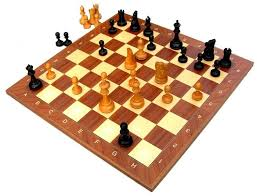
\includegraphics{./figure/chess.jpg}
\end{figure}
\end{frame}
\begin{frame}{Distributional Hypothesis}
\begin{itemize}
    \item<1-> words that occur in the same contexts tend to have similar meanings (Harris, 1945)
    \item<2-> how can we model the distributional hypothesis?
\end{itemize}
\end{frame}
\begin{frame}{Word-Context Matrix}
\begin{itemize}
    \item<1-> we count how often a word has occurred with a context in texts from a large corpus
    \item<2-> context is defined by a window over words
    \item<3-> let $V$ be the set of words in vocabulary and $C$ be the set of possible contexts
    \item<4-> word-context matrix $M$ is a two dimensional matrix whose rows are associated with $V$ and columns with $C$
    \item<5-> each entry of the matrix indicates how often a word co-occurs with a context in the given corpus
    \item<6-> this matrix is also known as co-occurrence matrix
\end{itemize}
\end{frame}
\begin{frame}{Word-Context Matrix}
\begin{itemize}
    \item corpus:
\begin{itemize}
    \item I like DL
    \item I like NLP
    \item I love ML
    \item I love NLP
\end{itemize}
\item window size = 1

\end{itemize}
\uncover<2->
{
\begin{table}[!h]
    \centering
    \begin{tabular}{l|cccccc}
          &  I & like & love & DL & NLP &ML  \\
          \hline
         I & 0 & 2 & 2 & 0 &0 &0  \\
         like & 2 & 0 & 0 & 1 & 1 &0 \\
         love & 2 & 0 & 0 & 0 & 1 & 1 \\
         DL & 0 & 1 & 0 & 0 & 0 & 0 \\
         NLP & 0 & 1 & 1 & 0 & 0  & 0\\
         ML & 0 & 0 & 1 & 0 & 0 & 0\\
         \hline
    \end{tabular}
\end{table}
}
\end{frame}


\begin{frame}{Word-Context Matrix}
\begin{itemize}
    \item corpus:
\begin{itemize}
    \item I like DL
    \item I like NLP
    \item I love ML
    \item I love NLP
\end{itemize}
\item window size = 1

\end{itemize}
\uncover<1->
{
\begin{table}[!h]
    \centering
    \begin{tabular}{l|cccccc}
          &  I & like & love & DL & NLP &ML  \\
          \hline
         I & 0 & 2 & 2 & 0 &0 &0  \\
         \textcolor{myblue}{like} & \textcolor{myblue}{2} & \textcolor{myblue}{0} & \textcolor{myblue}{0} & \textcolor{myblue}{1} & \textcolor{myblue}{1} & \textcolor{myblue}{0} \\
         \textcolor{red}{love} & \textcolor{red}{2} & \textcolor{red}{0} & \textcolor{red}{0} & \textcolor{red}{0} & \textcolor{red}{1} & \textcolor{red}{1} \\
         DL & 0 & 1 & 0 & 0 & 0 & 0 \\
         NLP & 0 & 1 & 1 & 0 & 0  & 0\\
         ML & 0 & 0 & 1 & 0 & 0 & 0\\
         \hline
    \end{tabular}
\end{table}
}
\end{frame}

\begin{frame}{Count-based Embeddings}
    \begin{itemize}
        \item<1-> for a large corpus, the size of matrix is very large 
        \item<2-> the matrix could be sparse too
        \item<3-> to encounter this, we may use dimensionality reduction techniques 
        \item<4-> however, for adding a new word we need to enlarge the matrix and apply dimensionality reduction again
    \end{itemize}
\end{frame}
\begin{frame}{CBoW Method}
    \begin{itemize}
        \item CBoW stands for Continuous Bag of Words
        \item task: given a context $\rightarrow$ predict a missing word from the context
        
            \begin{table}
                \begin{tabular}{l}
                    
                    input: ``I $\_$ NLP'' $\rightarrow$ output: ``like''   
                    \\
                    \\
                    \uncover<2->
                    {
                        input: (``I $\_$ NLP'', ``like'') $\rightarrow$ output: 1 and \\ 
                        input: (``I $\_$ NLP'', ``apple'') $\rightarrow$ output: 0
                    }
                \end{tabular}
            \end{table}
    \end{itemize}
\end{frame}
\begin{frame}{CBoW Method}
    \begin{itemize}
        \item<1-> given a corpus, we create two sets:
            \begin{itemize}
                \item<2-> positive set ($D$): consisting of pairs $(c, w)$ where $c$ is a context and $w$ is the correct value for the missing word
                \item<3-> negative set ($D^\prime$): consisting of pairs $(c, w)$ where $c$ is a context and $w$ is a random value for the missing word
            \end{itemize}
            \item<4-> we compute the score estimating similarity between context $c$  and word $w$ given context-word pair $(c,w)$
        \begin{equation*}
            s(c,w) = e(w)\sum_{w_i \in c} e(w_i)
        \end{equation*}
        where $e$ is a function that maps each word to its embeddings
        \item<5-> example
        \begin{equation*}
            s(\text{I }\_\text{ NLP},\text{like}) = e(\text{like})(e(\text{I})+e(\text{NLP}))
        \end{equation*}
    \end{itemize}
\end{frame}
\begin{frame}{CBoW Method}
        \begin{itemize}
            
            \item<1-> we use the sigmoid function to map the score to a probability
            \begin{equation*}
                P(y=1|(c,w)) = \frac{1}{1+ e^{-s(c,w)}}
            \end{equation*}
            \item<2-> we should maximize:
            \begin{equation*}
                \frac{1}{|D|} \sum_{(c,w)\in D} P(y=1|(c,w)) + 
                \frac{1}{|D^\prime|} \sum_{(c,w)\in D^\prime} P(y=0|(c,w))
            \end{equation*}
            \uncover<3->
            {
            
            or minimize the following loss
            \begin{small}
            \begin{equation*}
                L(\Theta) =  -\frac{1}{|D|}\sum_{(c,w)\in D}\text{log}P(y=1|(c,w)) - \frac{1}{|D^\prime|}\sum_{(c,w)\in D^\prime}\text{log}P(y=0|(c,w))
            \end{equation*}
            \end{small}
            }
        \end{itemize}
\end{frame}
\begin{frame}{Skip-Gram Method}
\begin{itemize}
    \item<1-> we treat words of a context independent from each other
            \begin{equation*}
                P(y=1|(c,w)) = \prod_{c_i \in c} P(y=1|(w,c_i)) = \prod_{c_i \in c} \frac{1}{1+e^{-e(w)e(c_i)}}
            \end{equation*}
    \item<2-> loss in Skip-Gram is identical to that in CBoW
    \item<3-> we fine-tune parameters (word embeddings) using SGD
\end{itemize}
\end{frame}
\begin{frame}{CBoW and Skip-Gram}
    \begin{itemize}
        \item<1-> CBoW loses the order information between context's elements
        \item<2-> CBoW allows the use of variable-length contexts
        \item<3-> Skip-Gram decouples the dependence between context elements even further than CBoW
        \item<4-> Skip-Gram treats each context's element as an independent context
    \end{itemize}
\end{frame}
\begin{frame}{Context Matters!}
    \begin{itemize}
        \item<1-> context of a word translates to its surrounding words in a sentence or paragraph
        \item<2-> window-based context: for a word  we consider all words in a window of length $2m+1$ centred on the word as context
        \item<3-> the size of window: large windows tend to capture more topical similarities and small windows capture syntactic similarities 
        \item<4-> contexts can be defined based on text units, for example, words that occur in the same sentence, paragraph, or text
        \item<5-> contexts can also be defined based on syntax of a sentence for example using parse tree or dependency tree of a sentence
        \item<6-> contexts of a word can be foreign words that are aligned to the word in multilingual corpora
    \end{itemize}
\end{frame}
\begin{frame}{Word2Vec Software Package}
    \begin{itemize}
        \item<1-> the implementations of CBoW and Skip-Gram methods exist in Word2Vec
        \item<1-> \url{https://code.google.com/archive/p/word2vec/}
        \item<2-> Skip-Gram is more effective in practice
    \end{itemize}
\end{frame}
\begin{frame}{GLoVe (Pennington et al., 2014)}\begin{itemize}
    \item GloVe: Global Vectors for Word Representation
    \item GloVe is an unsupervised method for obtaining word embeddings
    \item GloVe aims at reconciling the advantages of corpus-wide co-occurrence counts and local context windows
    \item \url{https://nlp.stanford.edu/projects/glove/}
\end{itemize}
\end{frame}
\begin{frame}{Evaluating Word Embeddings}
\begin{itemize}
     \item<1-> intrinsic
     \begin{itemize}
         \item<2-> word similarity tasks
         \item<2-> word analogy tasks
     \end{itemize}
     \item<3-> extrinsic
     \begin{itemize}
        \item<4-> on a downstream NLP task, we compare the performance of two models that differ only in the word embeddings they use
         \item<5-> named entity recognition (NER): accuracy
         \item<6-> machine translation (MT): BLEU score
         \item<7-> summarization: ROUGE score
         \item<8-> information retrieval (IR): precision - recall - F1 score
     \end{itemize}
\end{itemize}
 \end{frame}
\begin{frame}{Word Similarity Tasks}
     \begin{itemize}
         \item<1-> similar words should have similar representations
         \item<1-> dataset: \url{http://alfonseca.org/eng/research/wordsim353.html}
         \item<2->  word-1 and word-2 $\rightarrow$ similarity score $\in$ [0, 10]
         \item<3-> our function $f()$ should map two words to a similarity score using the distance between the word vectors of the words 
         \item<4-> cosine similarity
         \begin{equation*}
             \text{sim}(w_i,w_j) = \frac{e(w_i) e(w_j)}{||e(w_i)||^2 ||e(w_j)||^2}
         \end{equation*} 
     \end{itemize}
 \end{frame}
\begin{frame}{Word Analogy Tasks}
     \begin{itemize}
         \item<1-> A is to B as C to ?
         \item<2-> Germany is to Berlin as France is to ?
         \item<2-> dataset:
         \url{http://download.tensorflow.org/data/questions-words.txt}
         \item<3-> capital-common-countries
         \begin{itemize}
             \item<3-> Athens Greece Baghdad  $\rightarrow$ Iraq
             \item<3-> Athens Greece Berlin  $\rightarrow$ Germany
         \end{itemize}
         \item<4-> family
        \begin{itemize}
            \item<4-> boy girl brother $\rightarrow$ sister
            \item<4-> brother sister dad $\rightarrow$ mom
        \end{itemize}
     \item<5-> currency, adj-to-adverb, comparative, ...
     \end{itemize}
 \end{frame}
\begin{frame}{Finding the Prototype of  \\ a Group of Words}
     \begin{itemize}
        \item<1-> if we have a group of words $g = \{ w_1, w_2, ..., w_k \}$
        \item<2-> the prototype of this group can be computed as follows
            \begin{equation*}
                \text{proto}(g) = \frac{1}{k} \sum_{i \in 1..k} e(w_i)
            \end{equation*}
            where $e$ maps a word to its  embeddings
     \end{itemize}
 \end{frame}
 
 \begin{frame}{Finding Similar Words}
     \begin{itemize}
              \item<4-> cosine similarity
         \begin{equation*}
             \text{sim}(w_i,w_j) = \frac{e(w_i) e(w_j)}{||e(w_i)||^2 ||e(w_j)||^2}
         \end{equation*} 
        \item words found by embedding-based similarities can be filtered with other types of word similarities 
     \end{itemize}
 \end{frame}
\begin{frame}{Short Text Similarities}
     
     \begin{itemize}
        \item<1->  $d_1 = \{ w^1_1, w^1_2, ..., w^1_m \}$ and $d_2 = \{ w^2_1, w^2_2, ..., w^2_n \}$
        \item<2-> 
            \begin{equation*}
                \text{sim}(d_1, d_2) = \frac{1}{m.n}\sum_{i = 1}^m \sum_{j=1}^{n} \text{cos} \left( e(w_i^1), e(w_j^2) \right)
            \end{equation*}
          
     \end{itemize}
 \end{frame} 

 \begin{frame}{Pre-Trained Embeddings}
\begin{itemize}
    \item Word2Vec
    \begin{itemize}
        \item trained on Google News (100 billion tokens)
    \end{itemize}
    \item GloVe
        \begin{itemize}
            \item trained on Wikipedia (6 billion tokens)
            \item trained on CommonCrawl (42 and 840 billion tokens)
            \item trained on Twitter (27 million tokens)
        \end{itemize}
    \item many other pre-trained embeddings for different languages 
        \begin{itemize}
            \item \url{https://fasttext.cc/docs/en/crawl-vectors.html}
        \end{itemize}
\end{itemize}
\end{frame}

\begin{frame}{Practical Hints}
     \begin{itemize}
         \item<1-> always try out different word embeddings (consider them as a hyperparameter)
         \item<2-> results may vary drastically with different embeddings
         \item<3-> consider source of corpora used to train word embeddings (larger is not always better, a smaller but more domain-focused can be more effective)
         \item<4-> consider what contexts  were used to define similarities 
         \item<5-> it's better to use the same tokenization and text normalization methods that  were used for creating word embeddings
     \end{itemize}
 \end{frame}

\begin{frame}{Embedding Layers in PyTorch}
     \begin{itemize}
         \item<1-> an embedding layer (a.k.a lookup table) maps a sequence of word IDs to a sequence of embedding vectors
         \item<2-> it uses a lookup table, which is a matrix with size $|V|\times d_{emb}$
         \item<3-> the $i$'th row of this matrix contains embeddings of $i$'th word in vocabulary $V$
         \item<4-> so the only thing we need to do is to replace a word with its index in vocabulary $\rightarrow$ a dictionary does this easily (word$\_$to$\_$ix)
     \end{itemize}
\end{frame}

\begin{frame}[fragile]{Embedding Layers in PyTorch}
    \tiny
     \begin{lstlisting}[language=Python]
    import torch
    import torch.nn as nn
    import torch.nn.functional as F
    import torch.optim as optim
    
    torch.manual_seed(1)
    
    word_to_ix = {"hello": 0, "world": 1}
    
    embeds = nn.Embedding(2, 5) 

    lookup_tensor = torch.tensor([word_to_ix["hello"]], dtype=torch.long)
    
    hello_embed = embeds(lookup_tensor)
    
    print(hello_embed)
    
    \end{lstlisting}
\end{frame}
 
 \begin{frame}[fragile]{Embedding Layers in PyTorch}
  \tiny
     \begin{lstlisting}[language=Python]
import torch
import torch.nn as nn

class EmbeddingLayer(nn.Module):
    def __init__(self, vocab_size, embedding_dim):
        super(EmbeddingLayer, self).__init__()
        self.embeddings = nn.Embedding(vocab_size, embedding_dim)
    
    def forward(self, inputs):
        embeds = self.embeddings(inputs)
        return embeds
\end{lstlisting}        

\end{frame}
 
\begin{frame}[fragile]{Embedding Layers in PyTorch}
  \tiny
     \begin{lstlisting}[language=Python]
    import torch
    import torch.nn as nn

    class EmbeddingLayer(nn.Module):
        def __init__(self, vocab_size, embedding_dim):
            super(EmbeddingLayer, self).__init__()
            self.embeddings = nn.Embedding(vocab_size, embedding_dim)
        
        def forward(self, inputs):
            embeds = self.embeddings(inputs)
            return embeds

    if __name__ == '__main__':
        model = EmbeddingLayer(voc_size=10, emb_size=3)
        inputs = [1,5]
        inputs_tenseor = torch.tensor(inputs, dtype=torch.long)
        
        emb_vectors = model(inputs_tenseor)
        
        print(f"the shape of emb vectors is {emb_vectors.shape}")            
    \end{lstlisting}
\end{frame}

\begin{frame}[fragile]{Using Pretrained Embedding Layers  \\ in PyTorch}
  \tiny
     \begin{lstlisting}[language=Python]
    import torch
    import torch.nn as nn

    class EmbeddingLayer(nn.Module):
        def __init__(self, vocab_size, embedding_dim, weights_matrix):
            super(EmbeddingLayer, self).__init__()
            self.embeddings = nn.Embedding(vocab_size, embedding_dim)
            
            self.embeddings.load_state_dict({'weight': weights_matrix})
        
         
        def forward(self, inputs):
            embeds = self.embeddings(inputs)
            return embeds
    \end{lstlisting}
\end{frame}
 
\begin{frame}[fragile]{Freezing Embedding Layers \\ in PyTorch}
 
  \tiny
     \begin{lstlisting}[language=Python]
    import torch
    import torch.nn as nn

    class EmbeddingLayer(nn.Module):
        def __init__(self, vocab_size, embedding_dim, weights_matrix, freeze=False):
            super(EmbeddingLayer, self).__init__()
            self.embeddings = nn.Embedding(vocab_size, embedding_dim)
            
            self.embeddings.load_state_dict({'weight': weights_matrix})
            
            
            if freeze:
                self.embeddings.weight.requires_grad = False
            
            
        def forward(self, inputs):
            embeds = self.embeddings(inputs)
            return embeds
    \end{lstlisting}
\end{frame}
 
\begin{frame}{Limitations}
 \begin{itemize}
     \item<1-> the algorithms discussed provide very little control over the kind of similarity they include
     \begin{itemize}
         \item<2-> ``cat'' is more similar to ``dog'' than to ``tiger'' as they both are pets
         \item<3-> ``cat'' is more similar to ``tiger'' than to ``dog'' as they both as felines
     \end{itemize}
     \item<4-> many of the trivial properties of words are ignored because people are less likely to mention known information than they are to mention novel one
     \begin{itemize}
         \item<5-> when people talk about ``white sheep'', they will likely prefer to use only ``sheep''
         \item<6-> for ``black sheep'', they are very likely to use color information ``black sheep''
         \item<7-> a model trained on texts only might easily misled by this
     \end{itemize}
 \end{itemize}
\end{frame}
\begin{frame}{Limitations}\begin{itemize}
     \item<1-> text corpora can easily be biased for better or worse $\rightarrow$  so word embeddings can become biased too
     \begin{itemize}
         \item<2-> gender and racial biases are very common
     \end{itemize}
     \item<3-> these word vectors are context independent
     \begin{itemize}
         \item<4-> in reality, there is no such a thing to have context independent word meaning
         \item<5-> some words have multiple sense e.g., ``bank'' may refer to a financial institution or to the side of a river
     \end{itemize}
 \end{itemize}
\end{frame}
 
%%%%%%%%%%%%%%%%%%%%%%%%%%%%%%%%%%
\begin{frame}{Summary}
    \begin{itemize}
        \item common features used for converting textual data into numerical vectors
        \item basics of word embeddings
            \begin{itemize}
                \item how to get them? 
                \item where to use them?
                \item how to use them?
            \end{itemize}
        \item limitations
    \end{itemize}
\end{frame}
\begin{frame}[c]
\begin{center}
\LARGE{Thank You!}
\end{center}
\end{frame}



\end{document}